\documentclass{article}
\usepackage{geometry}[a4paper, margin=1in]
\usepackage{graphicx}
\usepackage{float}
\usepackage{subfigure}
\title{Practical Submission Sheet}
\newcommand{\bb}[1]{\textbf{#1}}
\date{}
\begin{document}
	\maketitle
	\begin{tabular}{ll}
		\bb{Term}: 2020-1 & \bb{Submission Date}: \today\\
		\bb{Lecture Date}: September 4th, 2020. & \bb{Practical Number}: 5\\
		\bb{Course Code}: PHY249 & \bb{Section}: G2903\\
		\bb{Registration Number}: 11912610 & \bb{Roll No}: 03\\
		\bb{Student Name}: Aayush Arya & \\
	\end{tabular}
	
	\section*{Aim} Create a combinational logic system for a given truth table and create a boolean expression for the same.
	
	\section*{Concepts Learnt}
	Learnt how circuit combinations can be used to create any desired logic system. Learnt making use of both NAND logic and AOI logic. Made use of deMorgan's theorem and wrote a boolean expression for the logic in context.
	
	\section*{Key Observations \& Insights}
	Both AOI and NAND combination logic circuits were created for two logic systems $ A. \bar{B} .\bar{C} = 1$ and $\bar{A}.\bar{B}.C + A.\bar{B}.\bar{C} = 1$ and their corresponding truth tables were empirically verified.
	
	\section*{Application Areas}
	Boolean logic is the most important in all of computer devices, these days now extending to emerging technologies such as internet of things. 

	\section*{Report}
	Firstly, a boolean expression for the logic summarized in Table 1 was written.
	\begin{table}[H]
		\centering
		\begin{tabular}{|l|l|l|l|}
			\hline
			Input A & Input B & Input C & Output\\
			\hline
			0 & 0 & 0 & 0\\
			0 & 0 & 1 & 0\\
			0 &1 &0& 0\\
			0 & 1 & 0 & 0\\
			0 &1 & 1 & 0\\
			1 & 0 & 0 & 1\\
			1 &0 & 1 &0\\
			1 &1 &0 &0\\
			1 &1 &1 &0\\
			\hline
		\end{tabular}
	\caption{Truth table for the first logic system that was studied.}
	\end{table}
	
	The key point to note in the truth table is that the output is "high" only for $A=1, B=0, C=0$, and therefore a suitable boolean expression for this would be $$ A. \bar{B} .\bar{C} = 1$$
	
	From deMorgan's law $$ \bar{B}.\bar{C} = \overline{B+C}$$
	Therefore,
	$$ A.(\overline{B+C}) = 1$$
	Since dot corresponds to an AND operation and + corresponds to an OR logic, our concerned logic system involves an AND gate with $A$ and $\overline{B+C}$ as the inputs, where $\overline{B+C}$ itself is the output of a NOR gate over B and C.\\
	
	The required logic system was constructed as shown in Figure 1.
	
	\begin{figure}[H]
		\centering
		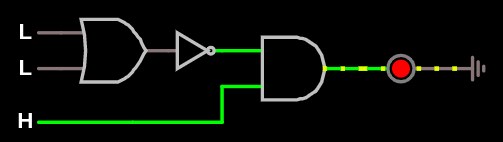
\includegraphics[width=0.8\textwidth]{AOI_1.png}
		\caption{AOI logic combination for the first truth table.}
	\end{figure}
	
	The truth tables were correspondingly verified. A NAND combination was also created for the same logic as shown in Figure 2.
	
	\begin{figure}[H]
		\centering
		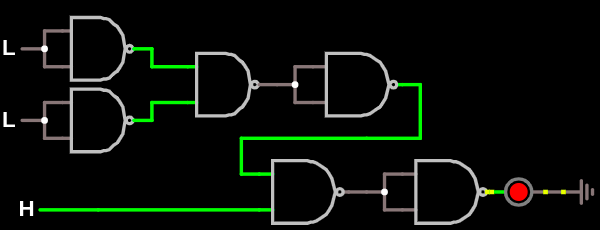
\includegraphics[width=0.8\textwidth]{NAND_1.png}
		\caption{A NAND combination for the concerned logic system.}
	\end{figure}

	Another logic system was studied, for which the given truth table was the following
	
	\begin{table}[H]
		\centering
		\begin{tabular}{|l|l|l|l|}
			\hline
			Input A & Input B & Input C & Output\\
			\hline
			0 & 0 & 0 & 0\\
			0 & 0 & 1 & 1\\
			0 &1 &0& 0\\
			0 & 1 & 0 & 0\\
			0 &1 & 1 & 0\\
			1 & 0 & 0 & 1\\
			1 &0 & 1 &0\\
			1 &1 &0 &0\\
			1 &1 &1 &0\\
			\hline
		\end{tabular}
		\caption{Truth table for the second logic system.}
	\end{table}
	
	The boolean expression for this logic system is $$\bar{A}.\bar{B}.C + A.\bar{B}.\bar{C} = 1$$
	
	An AOI logic combination equivalent to this boolean expression was created, as depicted in Figure 3. The truth table was also verified.
	\begin{figure}[H]
		\centering
		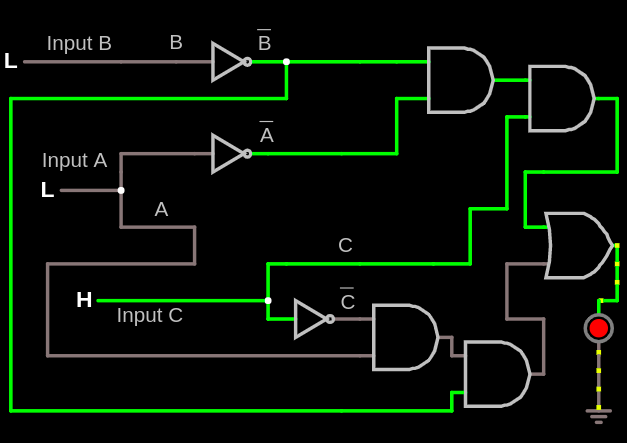
\includegraphics[width=0.8\textwidth]{AOI_2}
		\caption{AOI logic for the logic $\bar{A}.\bar{B}.C + A.\bar{B}.\bar{C}$}
	\end{figure}
\end{document}